\documentclass{ximera}

%\documentclass{ximera}

\usepackage{float}
\usepackage{subcaption}

\pgfplotsset{compat=1.16}

\newtheorem{ass}{Assumption}

\def\check{\tikz\fill[scale=0.4](0,.35) -- (.25,0) -- (1,.7) -- (.25,.15) -- cycle;}





\outcome{We continue to learn about the applications of the no arbitrage assumption.}

\author{Brad Waller}

%Section 2.5

\title{Inequalities}

\begin{document}

\begin{abstract}
Several fundamental inequalites are explored. They give us some powerful tools to analyze the price of calls and puts.
\end{abstract}

\maketitle

Last section, we worked with positions that had liabilities that perfectly matched. This match allowed us to use the positions to offset one another. This allowed us to infer values associated to other portfolios. Here, we will deal with portfolios that are simply compared to others to try to derive aggregate portfolios that have non-negative value (as opposed to zero value). There are three different portfolios that we will consider here; however, in the finance world, there are many more (many of which have bizarre names. 

The first portfolio we will consider is the bull spread. The idea of a bull spread is to buy a call and to write another call with a higher strike. The diagram below depicts a call with strike 20 and a written call with strike 30.


\begin{center}
	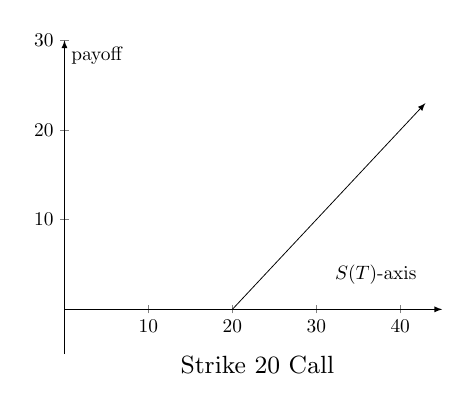
\begin{tikzpicture}[scale=0.7]
	\begin{axis}[
		xmin=0,
		xmax=45,
		%xtick={5,10,...,50},
		ymin=-5,
		ymax=30,
		%ytick={-20,-10,...,50},
		%grid=both,
		axis lines=middle,
		axis line style={->, >=latex},
		x label style={at={(0.95,0.2)}},
		%x label style={at={(axis description cs:0.86,0.42)},anchor=north},
		xlabel={$S(T)$-axis},
		ylabel={payoff}]
		%style={font=\tiny}]
		\addplot[black, smooth, domain=20:43, ->, >=latex]{x-20};
	\end{axis}
	\node at (3.5, -0.2) {\small Strike 20 Call};
	\end{tikzpicture}
	\hspace{10pt}
	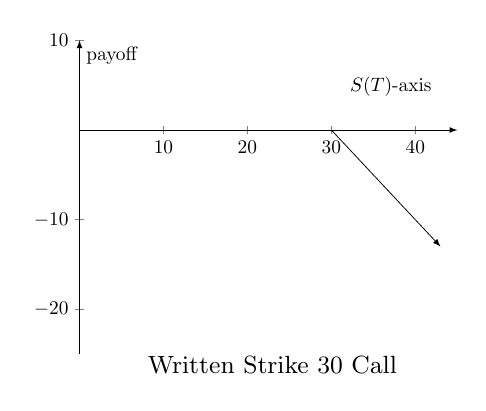
\begin{tikzpicture}[scale=0.7]
	\begin{axis}[
		xmin=0,
		xmax=45,
		%xtick={5,10,...,50},
		ymin=-25,
		ymax=10,
		%ytick={-20,-10,...,50},
		%grid=both,
		axis lines=middle,
		axis line style={->, >=latex},
		x label style={at={(0.95,0.8)}},
		xlabel={$S(T)$-axis},
		ylabel={payoff}]
		%style={font=\tiny}]
		\addplot[black, smooth, domain=30:43, ->, >=latex]{30-x};
	\end{axis}
	\node at (3.5, -0.2){\small Written Strike 30 Call};
	\end{tikzpicture}
\end{center}

The lazy approach from last section doesn't work as well since there are pieces of these functions that are both nonzero. Perhaps if we thought about these as piecewise functions first and added them together we would have better luck. The functions for each are
\begin{align*}
f_1(S)=\max\{S-20,0\}&=
	\begin{cases}
	S-20 	&	\text{if }S>20\\
	0	&	\text{otherwise,}
	\end{cases}\\
f_2(S)=-\max\{S-30,0\}&=
	\begin{cases}
	30-S 	&	\text{if }S>30\\
	0	&	\text{otherwise.}
	\end{cases}
\end{align*}
We can add these functions. We just have to remember to break this into three pieces. The only part that will be ``tricky'' wil be the values of $S$ larger than $30$.
\begin{equation*}
f_1(S)+f_2(S)=
	\begin{cases}
	S-20 	&	\text{if }20<S\leq 30\\
	10	&	\text{if }30<S\\
	0	&	\text{otherwise.}
	\end{cases}
\end{equation*}
I would probably never do this in practice. My view is that I only need to note the slopes of each function. Once I have that information, these functions become a lot easier to graph. In this problem, I would start with slope $0$ from $0$ to $20$. The slope would be $1$ from $20$ to $30$. Then the written call would contribute a negative one to the slope, bringing the sum's slope back to $0$ from $30$ to infinity. 

Let's graph the resulting function.

\begin{center}
	\begin{tikzpicture}[scale=0.7]
	\begin{axis}[
		xmin=0,
		xmax=45,
		%xtick={5,10,...,50},
		ymin=-5,
		ymax=25,
		%ytick={-20,-10,...,50},
		%grid=both,
		axis lines=middle,
		axis line style={->, >=latex},
		x label style={at={(0.95,0.20)}},
		%x label style={at={(axis description cs:0.86,0.42)},anchor=north},
		xlabel={$S(T)$-axis},
		ylabel={payoff}]
		%style={font=\tiny}]
		\addplot[black, smooth, domain=20:30, -, >=latex]{x-20};
		\addplot[black, smooth, domain=30:43,->, >=latex]{10};
	\end{axis}
	\node at (3.5, -0.2){\small Bull Spread};
	\end{tikzpicture}
\end{center}

Now, we can add one little dotted line to the picture that will reveal how this inequality will be realized.

\begin{center}
	\begin{tikzpicture}[scale=0.7]
	\begin{axis}[
		xmin=0,
		xmax=45,
		%xtick={5,10,...,50},
		ymin=-5,
		ymax=25,
		%ytick={-20,-10,...,50},
		%grid=both,
		axis lines=middle,
		axis line style={->, >=latex},
		x label style={at={(0.95,0.20)}},
		%x label style={at={(axis description cs:0.86,0.42)},anchor=north},
		xlabel={$S(T)$-axis},
		ylabel={payoff}]
		%style={font=\tiny}]
		\addplot[black, smooth, domain=20:30, -, >=latex]{x-20};
		\addplot[black, smooth, domain=30:43,->, >=latex]{10};
		\addplot[black, dotted, domain=0:43, -, >=latex]{10};
	\end{axis}
	\end{tikzpicture}
\end{center}

We see that our payoff diagram is always wedged between the values $0$ and $10$. This gives us the bull-spread inequality.
\begin{equation*}
0\leq c(20)-c(30)\leq \text{PV}(10)=10e^{-rT} 
\end{equation*}
In greater generality, we have that for strikes $K_1<K_2$
\begin{equation*}
0\leq c(K_1)-c(K_2)\leq (K_2-K_2)e^{-rT}
\end{equation*}
We could go further and say the following:
\begin{equation*}
0\leq c(K_1)-c(K_2)\leq \min\{c(K_1), (K_2-K_1)e^{-rT}\},
\end{equation*}
but it only makes things messier. One useful piece of information can be gleaned.
\begin{equation*}
c(K_1)\geq c(K_2)
\end{equation*}
That is to say, calls are alwasy non-increasing in value as a function of strike. This information is useful. 

We can apply everything we have done to puts. The difference is that we will need to buy the put with the higher strike and write the one with the lower strike. Please work out any of the details if they don't make sense.

\begin{center}
	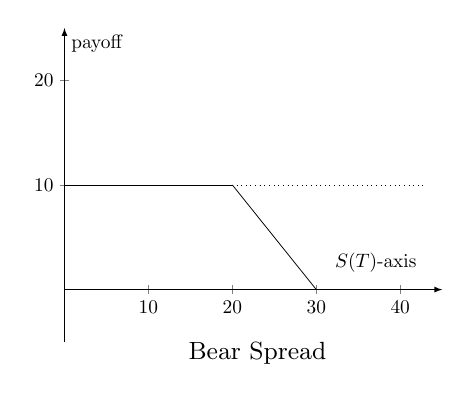
\begin{tikzpicture}[scale=0.7]
	\begin{axis}[
		xmin=0,
		xmax=45,
		%xtick={5,10,...,50},
		ymin=-5,
		ymax=25,
		%ytick={-20,-10,...,50},
		%grid=both,
		axis lines=middle,
		axis line style={->, >=latex},
		x label style={at={(0.95,0.20)}},
		%x label style={at={(axis description cs:0.86,0.42)},anchor=north},
		xlabel={$S(T)$-axis},
		ylabel={payoff}]
		%style={font=\tiny}]
		\addplot[black, smooth, domain=20:30, -, >=latex]{30-x};
		\addplot[black, smooth, domain=0:20,-, >=latex]{10};
		\addplot[black, dotted, domain=0:43,-,>=latex]{10};
	\end{axis}
	\node at (3.5, -0.2){\small Bear Spread};
	\end{tikzpicture}
\end{center}

This picture give almost the same information as the one used for the bull spread.
\begin{align*}
0&\leq p(K_2)-p(K_1)\leq (K_2-K_1)e^{-rT}\\
p(K_1)&\leq p(K_2)
\end{align*}
The second says that puts are always non-decreasing in value as a function of strike. We will use this fact later.

The last inequality we will develop comes from the butterfly spread. This opportunity is a little different than the previous ones. It uses only calls (or puts). Let's start with the diagram below.

\begin{center}
	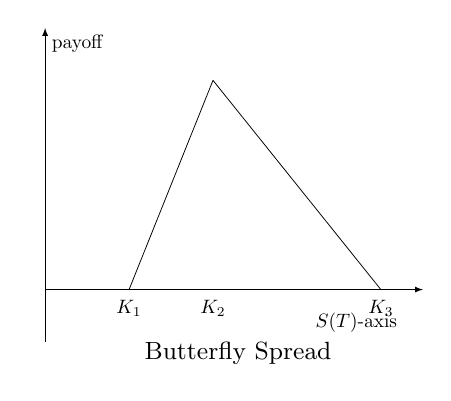
\begin{tikzpicture}[scale=0.7]
	\begin{axis}[
		xmin=0,
		xmax=45,
		xtick style={draw=none},
		xticklabels={,, $K_1$, $K_2$, , $K_3$},
		ymin=-5,
		ymax=25,
		ytick style={draw=none},
		yticklabels={,,},
		%grid=both,
		axis lines=middle,	
		axis line style={->, >=latex},
		x label style={at={(0.95,0.01)}},
		%x label style={at={(axis description cs:0.86,0.42)},anchor=north},
		xlabel={$S(T)$-axis},
		ylabel={payoff}]
		%style={font=\tiny}]
		\addplot[black, smooth, domain=10:20, -, >=latex]{2*(x-10)};
		\addplot[black, smooth, domain=20:40,-, >=latex]{20+(20-x)};
	\end{axis}
	\node at (3.5, -0.2){\small Butterfly Spread};
	\end{tikzpicture}
\end{center}

The payoff depicted here is never negative, and it is sometimes positive. This position should probably cost something. In addition, I have included three values. These should indicate strikes of some kind of option. The lack of labels gives me some freedom in my choices. I will begin by assuming that the first option is a call with strike $K_1$. This will match my diagram from $0$ to $K_2$. At $K_2$, an adjustment needs to be made. We need to determine that adjustment.

Since we purchased one call with strike $K_1$, the slope of our line connecting the points at $K_1$ and $K_2$ is 1. That means the value at the apex is $(K_2, K_1)$. We need to write a number of options so that the resulting line will connect the points $(K_2, K_1)$ and $(K_3,0)$. The slope of the line must be 
\[
-\frac{K_2-K_1}{K_3-K_2}.
\]

To move from a line with slope one to the line with slope we just mentions, we will need to write a number of options with strike $K_2$. That number is
\begin{equation*}
1+\frac{K_2-K_1}{K_3-K_2}=\frac{K_3-K_1}{K_3-K_2}.
\end{equation*}

If we stopped there, the diagram would be

\begin{center}
	\begin{tikzpicture}[scale=0.7]
	\begin{axis}[
		xmin=0,
		xmax=45,
		xtick style={draw=none},
		xticklabels={,, $K_1$, $K_2$, , $K_3$},
		ymin=-5,
		ymax=25,
		ytick style={draw=none},
		yticklabels={,,},
		%grid=both,
		axis lines=middle,	
		axis line style={->, >=latex},
		x label style={at={(0.95,0.01)}},
		%x label style={at={(axis description cs:0.86,0.42)},anchor=north},
		xlabel={$S(T)$-axis},
		ylabel={payoff}]
		%style={font=\tiny}]
		\addplot[black, smooth, domain=10:20, -, >=latex]{2*(x-10)};
		\addplot[black, smooth, domain=20:43,->, >=latex]{20+(20-x)};
	\end{axis}
	\end{tikzpicture}
\end{center}

We need to purchase some calls with strike $K_3$ to level things out. Fortunately, we know the slope of the line we are dealing with. We need to buy
\[
\frac{K_2-K_1}{K_3-K_2}
\]
calls with strike $K_3$ to level everything out. This gives us what we wanted.
\begin{align*}
c(K_1)-\frac{K_3-K_1}{K_3-K_2}c(K_2)+\frac{K_2-K_1}{K_3-K_2}c(K_3)&\geq0\\
c(K_1)+\frac{K_2-K_1}{K_3-K_2}c(K_3)&\geq \frac{K_3-K_1}{K_3-K_2}c(K_2)\\
\frac{K_3-K_2}{K_3-K_1}c(K_1)+\frac{K_2-K_1}{K_3-K_1}c(K_3)&\geq c(K_2)\\
\alpha c(K_1)+(1-\alpha)c(K_3)&\geq c(K_2)
\end{align*}
where $\alpha=\frac{K_3-K_2}{K_3-K_1}$. This relationships is different from the bull and bear spreads. It does not rely on time. This is simply a relationship regarding calls with various strikes. This also says that the price of a call is {\bf convex} or {\bf concave up} with respect to the strike. If we combine this with the bull spread information, we have an idea for what the price of a call should look like as we vary the strike.

In addition, we can use the same analysis to show that the result will also hold for put options. The value of $\alpha$ is the same as well.
\begin{equation*}
\alpha p(K_1)+(1-\alpha)p(K_3)\geq p(K_2)
\end{equation*}

Since this information is all important, let's group it all together into a theorem.

\begin{theorem}[Inequalities]
When our European call and put options have the same underlying asset and time to expiration, $T$, we have the following inequalities.
\end{theorem}
\begin{center}
	\renewcommand{\arraystretch}{1.8}
	\begin{tabular}{lc}
	Name of Relationship & Inequality\\
	\hline
	Bull Spread & $0\leq c(K_1)-c(K_2)\leq (K_2-K_1)e^{-rT}$\\
	Bear Spread & $0\leq p(K_2)-p(K_1)\leq (K_2-K_1)e^{-rT}$\\
	Butterfly Spread & $c(K_2)\leq \frac{K_3-K_2}{K_3-K_1}\cdot c(K_1)+\frac{K_2-K_1}{K_3-K_1}\cdot c(K_3)$\\
	Butterfly Spread & $p(K_2)\leq \frac{K_3-K_2}{K_3-K_1}\cdot p(K_1)+\frac{K_2-K_1}{K_3-K_1}\cdot p(K_3)$
	\end{tabular}
\end{center}

We would like to graph the calls and put with respect to their strikes, but we need a little more information. Let's answer the following questions:
\begin{itemize}
	\item What should the price of a strike $0$ call be?
	\item What should the price of a strike $0$ put be?
\end{itemize}

This isn't too difficult if you think of the payoffs. The call's will always be the underlying asset at expiration. That means the price of a strike $0$ call should be the prepaid forward price of the underlying asset. In contrast, the put's will always be $0$. That means the price of a strike $0$ put should be $0$. 

Now, we need one more piece of information for the graphs of call and put prices. We can call this an assumption for now. It may be something we can prove later under specific pricing models for calls and puts. 
\[
\lim_{K\to\infty}c(K)=0
\]

The figures below are cartoons of the reality, but they are certainly illustrative.

\begin{center}
	\begin{tikzpicture}[scale=0.7]
	\begin{axis}[
		xmin=-1,
		xmax=20,
		%xtick={5,10,...,50},
		ymin=-3,
		ymax=12,
		%ytick={-20,-10,...,50},
		%grid=both,
		axis lines=middle,
		axis line style={->, >=latex},
		x label style={at={(0.95,0.2)}},
		y label style={at={(.04,1)}},
		%x label style={at={(axis description cs:0.86,0.42)},anchor=north},
		xticklabels={,,},
		yticklabels={,,},
		xtick style={draw=none},
		ytick style={draw=none},
		xlabel={$K$-axis},
		ylabel={Call Price}]
		%style={font=\tiny}]
		\addplot[black, smooth, domain=0:18, ->, >=latex]{8*exp(-0.1*x)};
		\node[label={360:{$S(0)e^{-\delta T}$}},circle,fill,inner sep=2pt] at (axis cs:0,8) {};
	\end{axis}
	\node at (3.5, -0.2){\small Call Prices};
	\end{tikzpicture}
	\hspace{10pt}
	\begin{tikzpicture}[scale=0.7]
	\begin{axis}[
		xmin=-1,
		xmax=20,
		%xtick={5,10,...,50},
		ymin=-3,
		ymax=12,
		%ytick={-20,-10,...,50},
		%grid=both,
		axis lines=middle,
		axis line style={->, >=latex},
		xticklabels={,,},
		yticklabels={,,},
		xtick style={draw=none},
		ytick style={draw=none},
		x label style={at={(0.95,0.2)}},
		y label style={at={(.04,1)}},
		xlabel={$K$-axis},
		ylabel={Put Price}]
		%style={font=\tiny}]
		\addplot[black, smooth, domain=0:18, ->, >=latex]{x*exp(-0.03)+8*(exp(-0.1*x)-1)};
		\node[circle,fill,inner sep=2pt] at (axis cs:0,0) {};
	\end{axis}
	\node at (3.5, -0.2){\small Put Prices};
	\end{tikzpicture}
\end{center}

Another observation that we could make is that the put has a slant asymptote with slope $e^{-rT}$. This can be derived using put-call parity.

We've developed a lot of theory. Let's put it to practice!

\begin{example}
You are given the table below with various values of European calls and puts on the same underlying asset. The time to expiration is six months, and the risk-free rate is 7\%. Determine if there is an arbitrage opportunity present.
\end{example}
\begin{center}
	\begin{tabular}{lccc}
	Strike	&	45	&	50	&	55\\
	\hline	
	Call 	&	7.48	&	4.63	&	2.67\\
	Put	&	1.67	&	3.65	&	6.52
	\end{tabular}
\end{center}

\begin{solution}
There is a lot that we could do here: there are three pairs of bull spreads to check, three pairs of bear spreads to check, and two butterfly spreads to check. Let's just check one of each, and I will leave it to you to do the remainder. We'll check them in order.

Let's start with a bull spread consisting of one purchased call with strike 45 and one written call with strike 55.
	\begin{align*}
	c(45)-c(55)&\leq \text{PV}(10)\\
	7.48-2.67&\leq 10e^{-0.07\cdot 0.5}\\
	4.81&\leq 9.66\text{ \check}
	\end{align*}
There is no opportunity with that pair. Now let's try one of the bear spreads.
	\begin{align*}
	p(55)-p(50)&\leq \text{PV}(5)\\
	6.52-3.65&\leq 5e^{-0.07\cdot 0.5}\\
	2.87&\leq 4.83\text{ \check}
	\end{align*}
There is no opportunity with that pair. Finally, we will try a butterfly spread.
	\begin{align*}
	\alpha p(45)+(1-\alpha)p(55)&\geq p(50)\\
	0.5\cdot 1.67+0.5\cdot 6.52&\geq3.65\\
	4.095&\geq 3.65\text{ \check}
	\end{align*}
There is no opportunity with that butterfly spread. If you go and check the remaining 5 groupings of options, you will find that no opportunity exists!
\end{solution}

Now let's try a different kind of problem. This one will make you combine butterfly options with portfolio construction.

\begin{question}
You plan to use three different calls to construct the payoff diagram given below. 

\begin{center}
	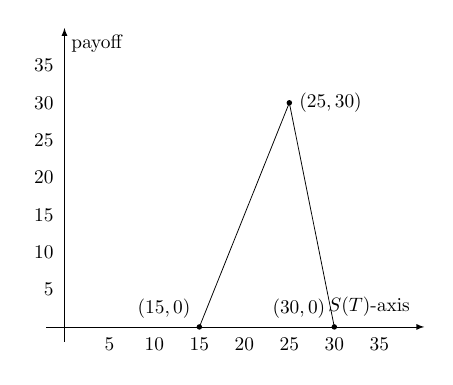
\begin{tikzpicture}[scale=0.7]
	\begin{axis}[
		xmin=-2,
		xmax=40,
		xtick style={draw=none},
		xtick={5, 10, ..., 35},
		ymin=-2,
		ymax=40,
		ytick style={draw=none},
		ytick={5, 10, ..., 35},
		%grid=both,
		axis lines=middle,	
		axis line style={->, >=latex},
		x label style={at={(0.98,0.06)}},
		%x label style={at={(axis description cs:0.86,0.42)},anchor=north},
		xlabel={$S(T)$-axis},
		ylabel={payoff}]
		%style={font=\tiny}]
		\addplot[black, smooth, domain=15:25, -, >=latex]{3*(x-15)};
		\addplot[black, smooth, domain=25:30,-, >=latex]{30+6*(25-x)};
		\node[label={360:{$(25,30)$}},circle,fill,inner sep=1pt] at (axis cs:25,30) {};
		\node[label={135:{$(15,0)$}},circle,fill,inner sep=1pt] at (axis cs:15,0) {};
		\node[label={135:{$(30,0)$}},circle,fill,inner sep=1pt] at (axis cs:30,0) {};
	\end{axis}
	\end{tikzpicture}
\end{center}

	\begin{prompt}
	\[
	\text{I should buy }\answer{3} \text{ calls with strike }15.
	\]
	\[
	\text{I should write }\answer{9} \text{ calls with strike } 25.
	\]
	\[
	\text{I should buy }\answer{6} \text{ calls with strike }30.
	\]
	\end{prompt}
	
\end{question}

\begin{solution}
It may seem that the numbers from the prompted response are arbitrary, but they can be deduced in a very clear way. The key here is to observe the slopes of your line segments. 

The first line segment connects the points $(15,0)$ and $(25,30)$. This line segment has slope 3. To arrive at this position, it is necessary to purchase 3 call options! The slope give you exactly what you need!

The second line segment connects the points $(25,30)$ and $(30,0)$. This line segment has slope -6. To go from a line with slope 3 to one with -6 requires you to write $(3-(-6))=9$ calls with strike 25.

The last part comes from eliminating the slope of -6. This requires you to buy 6 calls with strike 30! 

If any of this seems unclear, you can always write out the piecewise functions. This will never fail; however, it can be tedious.

In addition, we could have done this exact same portfolio using put options! It would have consisted of 6 puts with strike 30, 9 written puts with strike 25, and 3 puts with strike 15.
\end{solution}

\end{document}


\begin{question}
You are given that the price of some three-month European call and put are $2.83$ and $4.28$, respectively. The strike of the options is $72$. In addition, the underlying asset costs $70$ and has dividend rate $2\%$. What is the implied risk-free rate?

	\begin{prompt}
	\[	
	\text{The risk-free rate is }r=\answer{0.05}
	\]
	\end{prompt}
\end{question}

\begin{solution}
We must use put-call parity.
	\begin{align*}
	c-p&=S(0)e^{-\delta T}-Ke^{-rT}\\
	2.83-4.28&=70e^{-0.05}-72e^{-0.25r}\\
	72e^{-0.25r}&=71.10\\
	r&=0.05
	\end{align*}
\end{solution}

The main point of this section was to show that you can compare two seemingly different portfolios to get implied information regarding values of assets. This can lead to a variety of arbitrage opportunities. In the next section, we will extend this kind of reasoning to inequalities. The principle that will guide us is this: If a portfolio has only non-negative payoffs, then the position today must also be non-negative. 
\end{document}

